\documentclass{classrep}
\usepackage[utf8]{inputenc}
\usepackage{color}
\usepackage{gensymb}
\usepackage{listings}
\usepackage{tabto}
\usepackage{longtable}
\usepackage{graphicx}
\graphicspath{ {./pics/} }

\studycycle{Informatyka, studia niestocjanarne, I st.}
\coursesemester{IV}

\coursename{Systemy Wbudowane}
\courseyear{2019/2020}

\courseteacher{dr inż. Michał Morawski}
\coursegroup{Niedziela, 11:45-13:15}

\author{
  \studentinfo{KONRAD PŁAWIK}{191458} \and
  \studentinfo{Vladislav Mazur}{199185} \and
  \studentinfo{Łukasz Połubiński}{211833}
}

\title{Podlewaczka}
\svnurl{https://github.com/KP191458/Wbudowane}

\begin{document}
\maketitle
\newpage
\tableofcontents
\newpage

\section {Opis projektu}
Zadaniem projektu bylo stworzenie urządzenia które służyć będzie jako pomoc w monitorowaniu temperatury i wilgotności w ogrodzie bądź szklarni i dozowaniu zasobów wodnych. Urządznie mierzyć będzie temperaturę otoczenia i wilgotność powietrza. Pomierzone dane są wywietlane na ekranie a także urządzenie posiada dwie diody które sygnalizują przekrocznie ustalonego zakresu wilgotnosci. Przekroczenie zakresu uruchania także serwomechanizm, który może służyć jako urządzenie otwierające zawór nawodnienia szklarni.\\

\subsection {Wykaz urządzeń}
\begin{itemize} 
  \item Arduino Uno
  \item SHT31 - cyfrowy czujnik temperatury i wilgotności
  \item Arduino-Dem - moduł wyświetlacza LCD 2''
  \item Serwomechanizm Tower Pro SG90
  \item Diody LED 5 mm
  \item Rezystory przewlekane 330 \ohm
  \item Płytka stykowa 830 otworów
  \item Przewody połączeniowe męsko-męskie
  \item Przewody połączeniowe damsko-męskie
\end{itemize}

\subsection {Wykaz funkcjonalności}
\begin{enumerate}
  \item SPI
  \item GPIO
  \item Timer
  \item LCD
  \item SHT31 - temperatura
  \item SHT31 - wilgotność
  \item Serwomechanizm
  \item LED
\end{enumerate}

\section {Dokumentacja użytkownika}
\subsection {Wymagania sprzętowe}
Projekt wymagał xxxx co wymagało modelu Arduino który posiadał co najmniej taką ilość wejść i wyjść. Zdecydowalimy się na użycie Arduino Uno, ponieważ posiadało ono wymaganą liczbę wejść i wyjść oraz, ze względu na popularność posiadało liczne dokumentacje i przykłady użycia.

\subsection {Instrukcja użytkownika}
Po podłączeniu zasilania zainstalowane na urządzeniu oprogramowanie rozpoczyna inicjalizację urządzeń a następnie pomiar temperatury i wilgotności.

\begin{itemize}
  \item Pomiar wykonywany jest co 1 sekundę 
  \item Odczytane pomiary wywietlane są na wyświetlaczu LCD
  \item Dioda LED w kolorze zielonym informuje że zmieziona wilgotność jest poniżej 70\%.
  \item Dioda LED w kolorze czerwonym informuje że zmieziona wilgotność jest powyżej 70\%.
  \item Po przekroczeniu wilgotności 70\% uruchomiony zostaje serwomechanizm który wykorzystany może zostać do otwarcia zaworu systemu nawadniającego (w szklarni bądź pomieszczeniu)
\end{itemize}

\subsection {Interfejs użytkownika}
Urządzenie nie wymaga interakcji użytkownika w celu dokonania pomiarów. Interfejsem jest ekran oraz kolor diod LED.\\

Z ekranu możemy odczytać wartości liczbowe temperatury (w stopniach Celsjusza) oraz wilgotności (w procentach).

\section {Specyfikacja urządzeń}

\subsection {Arduino Uno}
Arduino Uno to płyta mikrokontrolera oparta na ATmega328. Posiada 14 cyfrowych wejść / wyjść (z których 6 można wykorzystać jako wyjścia PWM), 6 wejść analogowych, ceramiczny rezonator 16 MHz, złącze USB, gniazdo zasilania, nagłówek ICSP i przycisk resetowania.\\

Arduino Uno w wersji R3 to najnowsza wersja po Duemilanove, z ulepszonym układem interfejsu USB. Podobnie jak Duemilanove, ma on nie tylko rozszerzony nagłówek osłony z napięciem odniesienia 3,3 V i pin RESET (który rozwiązuje problem dotarcia do szpilki RESET w osłonie) oraz bezpiecznik 500 mA do ochrony portu USB komputera, ale także automatyczny obwód do wyboru zasilania USB lub DC bez zworki! Uno jest kompatybilny z kodami pin i Duemilanove, Diecimilla i starszymi Arduino, więc wszystkie płytki (shieldy), biblioteki i kod będą nadal działać. Nowy R3 (trzecia wersja) UNO ma kilka drobnych aktualizacji, z aktualizacją układu interfejsu USB i dodatkowymi przełamaniami dla pinów i2c i pinów IORef.\\

Arduino to platforma prototypowania elektroniki typu open source oparta na elastycznym, łatwym w użyciu sprzęcie i oprogramowaniu. Jest przeznaczony dla artystów, projektantów, hobbystów i wszystkich zainteresowanych tworzeniem interaktywnych obiektów lub środowisk.\\

Arduino może wyczuwać środowisko, otrzymując dane wejściowe z różnych czujników i może wpływać na otoczenie, kontrolując światła, silniki i inne siłowniki. Mikrokontroler na płycie programowany jest za pomocą języka programowania Arduino (opartego na Wiring) i środowiska programistycznego Arduino (opartego na Processing). Projekty Arduino mogą być autonomiczne lub mogą komunikować się z oprogramowaniem działającym na komputerze (np. Flash, Processing, Max / MSP).\\

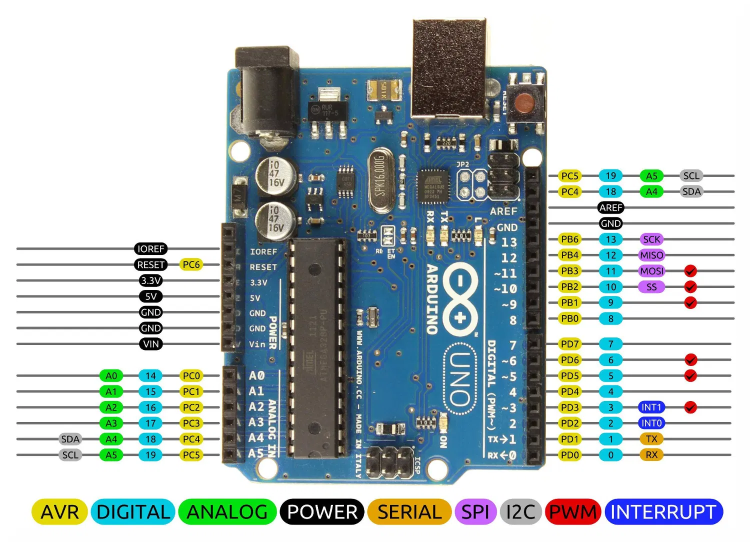
\includegraphics[scale=0.5]{Arduino-Uno}

Parametry techniczne:
\begin{itemize}
  \item Mikrokontroler ATmega328
  \item Napięcie robocze 5 V.
  \item Napięcie wejściowe (zalecane) 7-12 V.
  \item Napięcie wejściowe (limity) 6-20 V.
  \item Cyfrowe piny we / wy 14 (z których 6 zapewnia wyjście PWM)
  \item Piny wejścia analogowego 6
  \item Prąd DC na pin we / wy 40 mA
  \item Prąd DC dla 3,3 V Pin 50 mA
  \item Pamięć flash 32 KB (ATmega328) z czego 0,5 KB jest używane przez bootloader
  \item SRAM 2 KB (ATmega328)
  \item EEPROM 1 KB (ATmega328)
  \item Szybkość zegara 16 MHz
  \item Długość 68,6 mm
  \item Szerokość 53,4 mm
  \item Waga 25 g
\end{itemize}

\subsection {SHT31 - cyfrowy czujnik temperatury i wilgotności}
Seria czujników temperatury i wilgotności SHT3x dostępna jest w dwóch wersjach: wersja niskokosztowa SHT30 i wersja standardowa sht31. Rodzina SHT3x łączy wiele funkcji i interfejsów z przyjaznym szerokim zakresem napięć roboczych (2.4 do 5.5 V). W porównaniu do czujników poprzedniej generacji seria SHT3x jest inteligentniejsza, bardziej niezawodna i dokładniejsza. Jest bardziej funkcjonalny, ma wyższe możliwości przetwarzania sygnału i może odczytywać wartości temperatury i wilgotności za pomocą różnych pinów.\\

Ponadto wprowadzenie tej wersji dodatkowo rozszerzyło rodzinę produktów SHT3x. Zastosowanie osłony ochronnej typu filmowego rozszerza również zakres zastosowań. Jest to stopień ochrony IP67 dla wody i ochrona przeciwpyłowa niż folia PTFE, dzięki czemu może być stosowany w trudnych warunkach, w których woda i kurz mogą wpływać na dokładność i wydajność czujnika.\\

\begin{center}
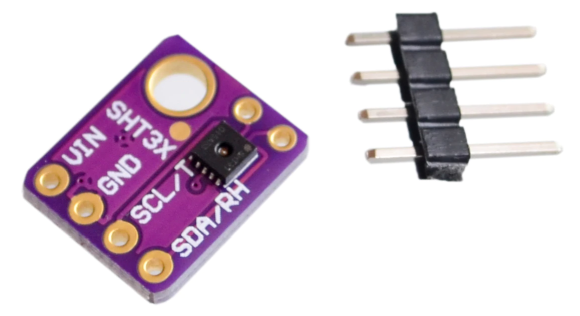
\includegraphics[scale=0.5]{SHT31}\\
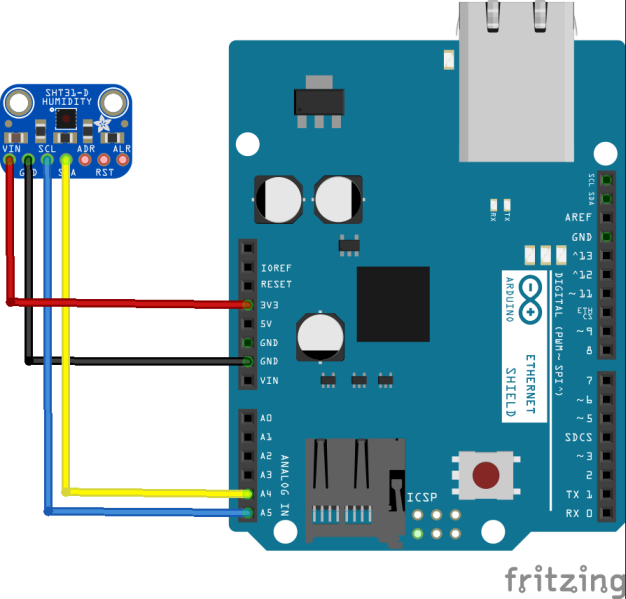
\includegraphics[scale=1.0]{SHT31-Arduino-Uno}
\end{center}

Cechy:
\begin{enumerate}
  \item Wysoka niezawodność i długa stabilność
  \item Z technicznego punktu widzenia niezawodne
  \item Nadaje się do aplikacji wysoka głośność
  \item Wysoka zdolność przetwarzania sygnału
  \item Niski poziom sygnału\\
\end{enumerate}


Parametry produktu:
\begin{enumerate}
  \item Wyjście: I2C, napięcie wyjściowe
  \item Napięcie zasilania: 2.4 do 5.5 V
  \item Zakres roboczy RH: 0-99.99\% RH
  \item Zakres temperatury pracy:-40 \degree do 125 \degree c (-40 \degree do 257 \degree f)
  \item Czas reakcji RH: 8 sekund (tau63 \%)
\end{enumerate}


\subsection {Arduino-Dem - moduł wyświetlacza LCD 2''}
DEM 1280640 FGH-PW\\

\begin{center}
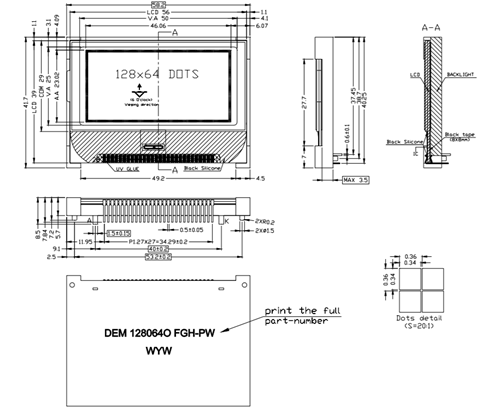
\includegraphics[scale=0.5]{U8G2}\\
\end{center}

FUNKCJE ORAZ CECHY\\
LCD TYPE
Transflective Positive Mode\\
Viewing Direction           : 6 o'clock\\
 Driving Scheme           : 1/65 Duty, 1/9 Bias\\
 Power Supply Voltage   : 3.3 Volt\\
 VLCD                        : 9.0 Volt\\
 Display Contents         : 128 x 64 Dots\\
 Driver IC                   : ST7565R (Sitronix)\\
 RoHS                        : Compliant\\
 Interfejs                    : SPI\\

SPECYFIKACJE MECHANICZNE\\
Module Size   	:  58.20 x 41.70 x 5.70 mm\\
Viewing Area 	:  50.00 x 25.00 mm\\
Active Area 	:  46.06 x 23.02 mm\\
Dot Size		: 20.34. x 0.34 mm\\
Dot Gap 		: 20.02 mm\\

\subsection {Serwomechanizm Tower Pro SG90}
9-gramowe serwo typu micro SG90 firmy TowerPro to bardzo popularny model serwa stosowany w modelarstwie, robotyce, konstrukcjach napędowych, systemach alarmowych.\\

Serwo ma niewielką wagę lecz jest stosunkowo szybkie i ma siłę odpowiednią do sterowania modelami.\\

\begin{center}
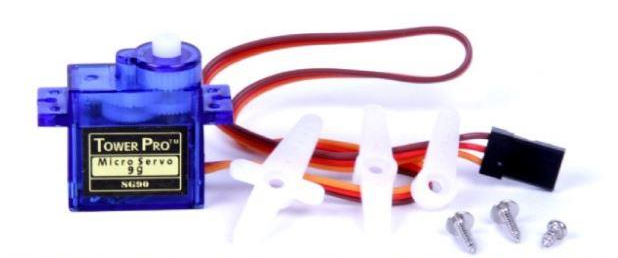
\includegraphics[scale=0.5]{SG90}\\
\end{center}

Charakterystyka:
\begin{itemize}
  \item Prędkość przekładni: 0,12 s/60\degree (4,8 V)
  \item Moment: 1,2 – 1,8kg/cm (4,8 V)
  \item Napięcie pracy: 4,8 – 7,2V
  \item Długość przewodów zasilania: 23,5cm
  \item Waga: 9g
  \item Czas reakcji: 7 us
  \item Temperatura pracy: -30 do +60 stopni
  \item Wymiary 22mm x 12mm x 22,7mm\\
\end{itemize}

Oznaczenie przewodów:
\begin{itemize}
  \item Czerwony: zasilanie
  \item Brązowy: masa
  \item Pomarańczowy: sygnał
\end{itemize}

\subsection {Diody LED 5 mm}
Parametry diody zielonej:
\begin{itemize}
  \item Soczewka w kolorze zielonym
  \item Obudowa: DIP 5 mm
  \item Długość emitowanej fali: 571 nm
  \item Jasność: 100 - 150 mcd
  \item Kąt świecenia: 50\degree
  \item Temp. pracy: od-40 \degree C do +80 \degree C
  \item Parametry pracy:
\begin{itemize}
  \item Prąd If: 20 mA
  \item Napięcie Vf: 2,3 - 2,5 V\\
\end{itemize}
\end{itemize}

Parametry diody czerwonej:
\begin{itemize}
  \item Soczewka w kolorze czerwonym
  \item Obudowa: DIP 5 mm
  \item Długość emitowanej fali: 625-645 nm
  \item Jasność: 450 - 800 mcd
  \item Kąt świecenia : 70 \degree
  \item Temp. pracy: od -40 \degree C do +80 \degree C
  \item Parametry pracy:
\begin{itemize}
  \item Prąd If: 20mA
  \item Napięcie Vf: 2,0 - 2,3 V'
\end{itemize}
\end{itemize}

\subsection {Rezystor przewlekany 330 \ohm}
Specyfikacja rezystorów
\begin{itemize}
  \item Rezystancja: 330 \ohm
  \item Moc znamionowa: 1/4 W
  \item Tolerancja: 5\%
  \item Montaż: przewlekany THT
\end{itemize}
\subsection {Płytka stykowa 830 otworów}
Dane techniczne płytki stykowej
\begin{itemize}
  \item Wymiary: 165 x 53 mm
  \item Liczba otworów: 830
  \item Posiada kolorowe paski, które mogą oznaczać polaryzację zasilania (+i-)
\end{itemize}

\section {Specyfikacja funkcjonalności}
\subsection {SPI}
Interfejs SPI( Serial Peripheral Interface) używany jest do komunikacji z wyświetlaczem i diodami LED. Inicjalizacja obsługi wyświetlacza odbywa się poprzed załącznie biblioteki oraz wywołanie konstruktora identyfikującego urządzenie. W naszym wypadku jest to:\\ U8G2\_ST7567\_ENH\_DG128064\_F\_4W\_SW\_SPI\\

Przekazujemy do niego następujące wartości:\\
\textbf{rotation}: czyli kąt obrotu zawartości wyświetlacza (w naszym wypadku 180 stopni)\\
\textbf{SCL} (clock): numer pinu timera (sygnał taktujący) (PIN 13)\\
\textbf{SDA} (data): numer pinu przesyłu danych (PIN 11)\\
\textbf{CS}: wybór układu podrzędnego (PIN 10)\\
\textbf{D/C} (dc): numer pinu odpowiedzialny za wybór pomiędzy trybem instrukcji a trybem zanków (PIN 9)\\
\textbf{reset}: numer pinu odpowiedzialny za restart ekranu (PIN 8)\\

clock, data, cs, dc, reset mają wartości jednobajtowe.\\
\subsection {GPIO}
GPIO (General Purpose Input/Output) . GPIO kontroluje piny, ustawiając ich stan na wysoki (1 - HIGH) lub
niski (0 - LOW) co, odpowiednio, skutkuje ustawieniem pina na urządzenia wyjścia jak i wejścia.
W projekcie naszym użylimy GPIO do zmiany stanu dwóch diod LED sygnalizujących kolorem poziom wilgotności. 

Fragmenty kodu podpowiadające za użycie GPIO:
\begin{lstlisting}
int czerwona = 7;
int zielona = 6;

pinMode(czerwona, OUTPUT);
pinMode(zielona, OUTPUT);

  if(h>70.0)
  {
    digitalWrite(czerwona, HIGH);
    digitalWrite(zielona, LOW);
  }
  else
  {
    digitalWrite(czerwona, LOW);
    digitalWrite(zielona, HIGH);
  }
\end{lstlisting}

\subsection {LCD}
Użyta przez nas funkcjonalność niezbędna do podstawowej obsługi wyświetlacza przedstawiona została w rozdziale dotyczącym SPI. Natomiast jeśli zajdzie taka potrzeba można dokonać zaawansowanej obsługi wywietlacza poprzez wpisanie porządanych wartości w konkretne rejestry urządzenia. \\

Architekturę urządzenia przedstawia diagram:\\
\begin{center}
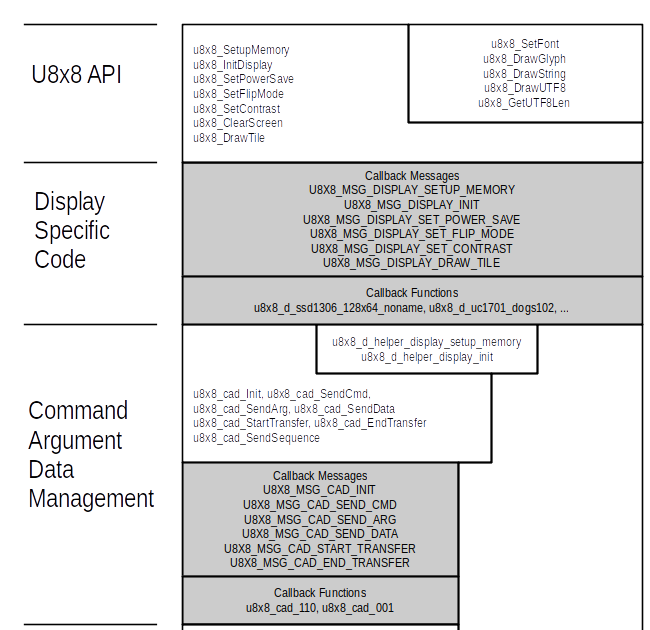
\includegraphics[scale=0.5]{u8g2_software_architecture1}\\
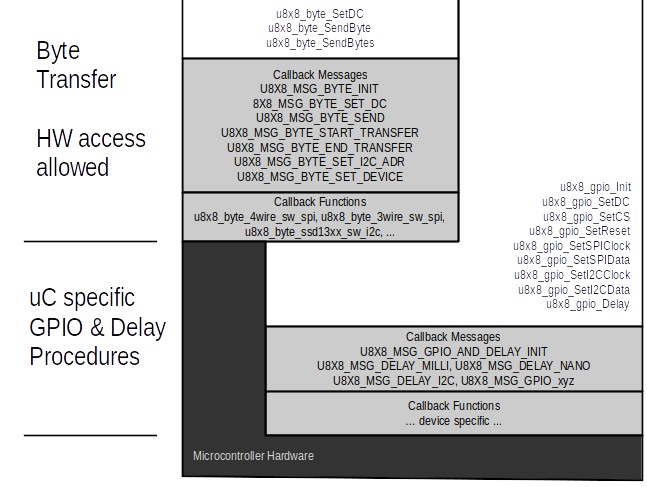
\includegraphics[scale=0.5]{u8g2_software_architecture2}
\end{center}

Pełna lista rejestrów cmds znajduje się pod adresem:\\
\url{https://github.com/olikraus/u8g2/blob/master/doc/controller_cmds.txt}

Najważniejsze z nich to:\\

\begin{center}
\begin{longtable}{ c c c }
0x000 & 00000000 & Lo Col \\
0x00f & 00001111 & Lo Col \\
0x010 & 00010000 & Hi Col \\
0x01f & 00011111 & Hi Col \\
0x020 & 00100000 & Res Ratio \\
0x023 & 00100011 & Res Ratio \\
0x024 & 00100100 & Res Ratio \\
0x027 & 00100111 & Res Ratio \\
0x028 & 00101000 & Pwr Ctrl \\
0x02f & 00101111 & Pwr Ctrl \\
0x040 & 01000000 & Start Line \\
0x07f & 01111111 & Start Line \\
0x081 & 10000001 & Contrast \\
0x0a0 & 10100000 & Seg Normal \\
0x0a1 & 10100001 & Seg Reverse \\
0x0a2 & 10100010 & 1/9 bias \\
0x0a3 & 10100011 & 1/7 bias \\
0x0a4 & 10100100 & Normal Op \\
0x0a5 & 10100101 & All pt on \\
0x0a6 & 10100110 & Normal Op \\
0x0a7 & 10100111 & Inverse \\
0x0ac & 10101100 & Indic. On \\
0x0ad & 10101101 & Indic. Off \\
0x0ae & 10101110 & Disp Off \\
0x0af & 10101111 & Disp On \\
0x0b0 & 10110000 & Page Adr \\
0x0b7 & 10111111 & Page Adr \\
0x0c0 & 11000xxx & Com Normal \\
0x0c7 & 11000xxx & Com Normal \\
0x0c8 & 11001xxx & Com Reverse \\
0x0cf & 11001xxx & Com Reverse \\
0x0e0 & 11100000 & Start R-M-W \\
0x0e2 & 11100010 & Reset
\end{longtable}
\end{center}
\subsection {I2C}
Magistrala I2C zawiera siedem rejestrów:
\begin{itemize}
  \item \textbf{I2CONSET} (Control Set register) Odpowiada za ustawianie bitów w rejestrze I2CON, który
kontroluje operacje na interfejsie I 2 C. Ustawienie jedynki w tym rejestrze skutkuje
ustawieniem odpowiedniego bitu w rejestrze kontrolnym I 2 C. Ustawienie stanu niskiego
(zera) nie powoduje żadnych efektów. I2CONSET zawiera osiem bitów.
  \item \textbf{I2STAT} (Status register) Odpowiada za informacje o I 2 C, rejestr w trybie tylko do odczytu.
Również posiada osiem bitów, z czego trzy pierwsze (bity o numerze 0,1,2) są nieużywane i
są zerami. Pozostałe bity o numerach 3,4,5,6,7 dostarczają informacji statusie interfejsu I 2 C.
  \item \textbf{I2DAT} (Data register) Rejestr ten zawiera wysłane lub otrzymane dane. Proces może
odczytać i zapisywać ten rejestr tylko wtedy, gdy nie jest w trakcie przesuwania bitu
  \item \textbf{I2ADR} (Slave Address register) Rejestr ten jest możliwy do odczytu i zapisu. Używany tylko
wtedy, gdy interfejs I 2 C jest ustawiony na slave mode. W innym przypadku rejestr nie jest
używany.
  \item \textbf{I2SCLH} (High duty cycle register) Rejestr ten zawiera 16 bitów (od 0 do 15). Ustawia czas SCL
HIGH zegara I 2 C.
  \item \textbf{I2SCLL} (Low duty cycle register) Rejestr ten zawiera 16 bitów (od 0 do 15). Ustawia czas SCL
LOW zegara I 2 C.
  \item \textbf{I2CONCLR} (Control Clear register) Odpowiada za czyszczenie bitów w rejestrze I2CON.
Ustawienie jedynki w tym rejestrze skutkuje ustawieniem odpowiedniego bitu w rejestrze
kontrolnym I 2 C. Ustawienie zera nie powoduje żadnych efektów. Rejestr ten posiada osiem
bitów.\\
\end{itemize}
W projekcie naszym używaliśmy jedynie rejestru \textbf{I2ADR}.

\subsection {SHT31}
Odczyt z termometru/miernika wilgotności SHT31 opiera się o odczyt danych z wymienionego wyżej rejestru I2ADR. Do zaawansowanej obsługi SHT31 możemy użyć jego rejestrów:

\begin{center}
\begin{longtable}{ c c c }
nazwa & wartość & opis \\
SHT31\_DEFAULT\_ADDR & 0x44 & Adres domyślny \\
SHT31\_MEAS\_HIGHREP\_STRETCH & 0x2C06 & Measurement High Repeatability \\
 &  & with Clock Stretch Enabled \\
SHT31\_MEAS\_MEDREP\_STRETCH & 0x2C0D & Measurement Medium Repeatability \\
 &  & with Clock Stretch Enabled \\
SHT31\_MEAS\_LOWREP\_STRETCH & 0x2C10 & Measurement Low Repeatability \\
 &  & with Clock Stretch Enabled \\
SHT31\_MEAS\_HIGHREP & 0x2400 & Measurement High Repeatability \\
 &  & with Clock Stretch Disabled \\
SHT31\_MEAS\_MEDREP & 0x240B & Measurement Medium Repeatability \\
 &  & with Clock Stretch Disabled \\
SHT31\_MEAS\_LOWREP & 0x2416 & Measurement Low Repeatability \\
 &  & with Clock Stretch Disabled \\
SHT31\_READSTATUS & 0xF32D & Read Out of Status Register \\
SHT31\_CLEARSTATUS & 0x3041 & Clear Status \\
SHT31\_SOFTRESET & 0x30A2 & Soft Reset \\
SHT31\_HEATEREN & 0x306D & Heater Enable \\
SHT31\_HEATERDIS & 0x3066 & Heater Disable \\
SHT31\_REG\_HEATER\_BIT & 0x0d & Status Register Heater Bit  \\
\end{longtable}
\end{center}

\subsection {Serwomechanizm}
Serwomechanizm wykorzystuje interfejs SPI. Obsługa serwomechanizmu odbywa się za pomocą bilioteki Servo. Przy inicjalizacji przypisujemy numer pinu a następnie przy pomocy funkcji write podajemy kąt jaki wskazać ma serwomechanizm.

\subsection {LED}
Diody LED wykorzystują jedynie GPIO oraz w/w funkcje: pinMode i digitalWrite.

\section{Analiza skutków awarii}
\subsection {Arduino Uno}
Skutek awarii: \textbf{Krytyczny}\\
W przypadku awarii, uszkodzenia lub braku zasilania mikrokontrolera nie ma możliwości skorzystania z całego urządzenia. Problemy z bootowanie bądź brakiem zasilania zdarzały się często i koniecny był wtedy restart całego układu. Błąd nie występował podczas prac nad projektem.
\subsection {Interfejs SPI}
Skutek awarii: \textbf{Krytyczny}\\
W przyapdku awarii interfejsu SPI mamy pomiar temperatury ale nie mamy możliwości skorzystania z wyświetlacza, diod LED czy serwomechnizmu. Pomiar możemy odczytać wtedy jedynie na konsoli aplikacji Arduino ale nie jest to wystarczające dla docelowego użytkownika. Błąd nie występował podczas prac nad projektem.
\subsection {Interfejs I2C}
Skutek awarii: \textbf{Krytyczny}\\
W naszym wypadku tożsamy z brakiem odczytu temperatury i poziomu wilgotności czyli uniemożliwia działanie systemu.
\subsection {SHT31}
Skutek awarii: \textbf{Krytyczny}\\
Jak wyżej. Brak odczytu temperatury i poziomu wilgotności uniemożliwia działanie całego systemu. Błąd raczej rzadko występujące.
\subsection {Wyświetlacz LCD}
Skutek awarii: \textbf{Średni}\\
Brak samego wyświetlacza pozwoli na działanie projektu - diody zasygnalizują przekroczenie poziomu wilgotności a serwomechanizm odkręci zawód. Błąd wystąpił kilka razy ale klasyfikuje go jako raczej rzadko występujący.
\subsection {Serwomechanizm}
Skutek awarii: \textbf{Średni}\\
Brak samego serwomechanizmu pozwoli na działanie projektu - diody zasygnalizują przekroczenie poziomu wilgotności a dokładne wartości wyświetlone będą na wyświetlaczu. Błąd wystąpował dosyć często ze wszględu na znaczną konsumpcje napięcia przez serwomechanizm.
\subsection {Diody LED}
Skutek awarii: \textbf{Niski}\\
Brak działających diod LED nie wpływa na działanie projektu - jest to łatwo widoczny sygnał dla użytkownika ale nie jest to niezbędny element do działania pozostałych komponentów.

\section{Awaryjność w czasie}
Ze względu na konieczność długotrwałego działania, podczas tworzenia projektu układ poddaliśmy testom aby ocenić wpływ czasu na jego działanie. Układ pozostawiliśmy właczony przez dwa kilkudniowe okresy i podczas tego czasu działał on stabilnie i bezawaryjnie - temperatura i wilgotność były mierzone, wyświetlacz wskazywał pomiary a diody sysgnalizowały poziom.

\begin{thebibliography}{0}
\end{thebibliography}
\url{https://github.com/adafruit/Adafruit_SHT31/}\\
\url{https://github.com/olikraus/u8g2/tree/master/doc}\\
\url{http://www.fis.agh.edu.pl/~skoczen/embed/pdf3/I2C_LPC17xx.pdf}\\
\end{document}
